\cleardoublepage
\newpage
\section*{DISCUSIÓN}
\addcontentsline{toc}{section}{DISCUSIÓN}
\par\refstepcounter{section}
\subsection{Pruebas en proteínas}
\par
La primera prueba que se le hace a los nuevos potenciales BSASA y SASA es la clasificación de estructuras en nativas y no nativas, un problema considerado ya resuelto por una gran cantidad de software y métodos publicados. (citar metodos)
En la figura~\ref{fig:ferrada2009} podemos observar como los potenciales de la metodología nueva utilizando subsuperfices y la combinación con potenciales de superfície tienen peores resultados que los que utilizan distancias y la combinación de conteo de átomos y distancia.
Esto se debe al rango de interacción más corto que tienen los potenciales BSASA, que impide el reconocomiento de posibles interacciones no favorables más distantes (figura~\ref{fig:radii_int}) que no es capaz de observar ya que el rango máximo de distancia es equivalente a dos veces el radio de Van der Waals más 1.4 \si{\angstrom} de distancia, siendo 1.4 \si{\angstrom} el radio de una molécula de agua.
En la figura~\ref{fig:radii_int} podemos ver las distribuciones de la cantidad de interacciones entre pares de átomos para las estructuras utilizadas en la derivación de los potenciales en proteína.
\begin{figure}[!p]
\centering
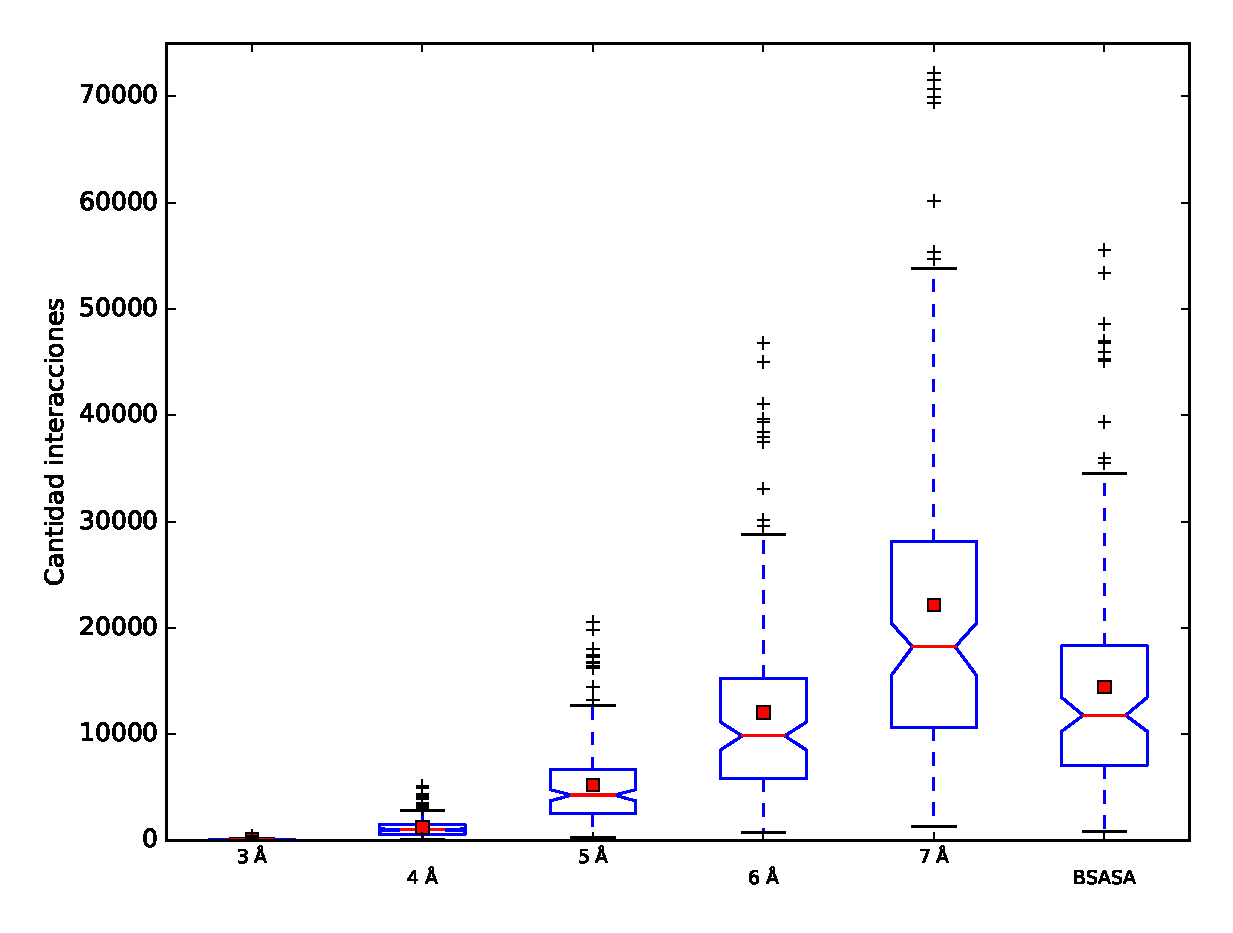
\includegraphics[width=\linewidth]{figures/radii_int.eps}
\caption[Boxplots de las distribuciones de la cantidad de contactos encontrados en el conjunto de estructuras usado en la derivación de potenciales para proteínas.]{Boxplots de las distribuciones de la cantidad de contactos encontrados en el conjunto de estructuras usado en la derivación de potenciales para proteínas. En la figura se tienen las distribuciones de la cantidad de contactos para potenciales dependientes de distancia variando el radio máximo de interacción de 3 a 7 \si{\angstrom}, más el potencial BSASA. La línea roja indica la mediana, el punto rojo el promedio, y la cintura el intervalo de confianza.}
\label{fig:radii_int}
\end{figure}
La distribución para BSASA muestra que el potencial evalua una menor cantidad de interacciones que los potenciales de distancia, que usan un rango de máximo de 7 \si{\angstrom} para evaluar interacciones.
De acuerdo a la ecuación~\ref{ec:ip} esto implica directamente que el potencial BSASA tiene un menor contenido de información disponible para la evaluación de la estructura, dado el menor número de interacciones pareadas observadas, que es el término \textit{n} en la ecuación.
Entre tanto, el potencial SASA logra un mucho mejor desempeño que conteo, dado que es mucho más fino en registrar si un átomo esta enterrado o expuesto, ya que se mide directamente la superficie en contacto con el solvente, en vez del método indirecto del potencial de conteo.
\par
En la segunda prueba, la capacidad de los nuevos potenciales BSASA y SASA en detectar errores aislados y expuestos en la superficie, tanto como errores más internos y difíciles de detectar fue evaluada utilizando perfiles de energía, en vez de usar el valor promedio de energía como en las pruebas anteriores.
Estos perfiles de energía contienen valores de energía promediados en una ventana deslizante de 7 residuos lo que permite eliminar variaciones bruscas en los valores de energía de cada residuo.
En esta prueba el valor final de energía de cada residuo se evalúa como un elemento independiente.
Al evaluar los errores de clase A, notamos que el desempeño de los pares de potenciales comparables no es distinguible, excepto en el caso de los potenciales SASA y CONTEO.
Dado que los errores en los residuos clase A son en residuos aislados y expuestos, el mejor desempeño de SASA versus CONTEO era esperado.
A su vez, los potenciales DD y BSASA y sus respectivas combinaciones DD+CONTEO y BSASA+SASA no muestran diferencias significativas en estos modelos.
Pero en los modelos clase B, cuyos residuos poseen errores más internos en la estructura afectando también residuos correctamente modelados su alrededor o entorno local, los potenciales BSASA y BSASA+SASA logran un desempeño superior a los potenciales DD y DD+CONTEO.
Esto se debe a la capacidad del potencial BSASA de excluir naturalmente los contactos que están escondidos detrás de otros átomos, algo que los potenciales de distancia no pueden detectar normalmente sin utilizar algoritmos para la detección de esos casos. (\cite{Ferrada2007,Ferrada2009})

\subsection{Pruebas en RNA}
En la primera prueba se observó la correlación del valor de energía calculado por los potenciales con las medidas de desviación estructural de más de 80 estructuras con 500 modelos cada una.
Esta prueba es muy similar a la primera prueba en proteínas, que buscaba separar modelos entre nativos y no nativos, que no es aún posible realizar dada la falta de una base de datos de estructuras y modelos de ARN ya clasificados en nativos y no nativos.
Al igual que en la primera prueba en proteínas, los potenciales BSASA y su combinación BSASA+SASA tienen un desempeño menor al potenciale de referencia RASP.
El potencial RASP utiliza un rango de 10 \si{\angstrom} para la detección de interacciones, lo que significa que es capaz de detectar y evaluar motifs de estructuras terciarias estadisticamente probables de estar en proximidad.
En la figura~\ref{fig:radii_rna}
